% Q20 -- Scannable flip-flop in scannable register design: D flip-flop preceded by a
% 2:1 mux. SCAN deasserted -> stores D (normal); SCAN asserted -> loads SI (scan chain).
\documentclass[border=10pt]{standalone}
\usepackage{tikz}
\usetikzlibrary{arrows.meta,shapes.geometric}
\begin{document}
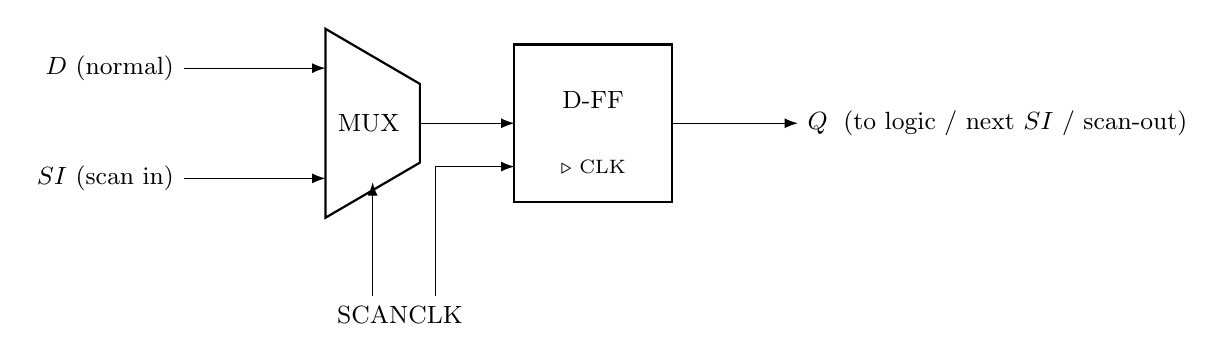
\begin{tikzpicture}[>=Latex, font=\small]
% 2:1 mux as a trapezoid
\draw[thick] (0,0) -- (0,2.4) -- (1.2,1.7) -- (1.2,0.7) -- cycle;
\node at (0.55,1.2) {MUX};
\draw[->] (-1.8,1.9) node[left]{$D$ (normal)} -- (0,1.9);
\draw[->] (-1.8,0.5) node[left]{$SI$ (scan in)} -- (0,0.5);
\draw[->] (0.6,-1.0) node[below]{SCAN} -- (0.6,0.45);
% D flip-flop
\draw[thick] (2.4,0.2) rectangle (4.4,2.2);
\node at (3.4,1.5) {D-FF};
\node[font=\scriptsize] at (3.4,0.65) {$\triangleright$ CLK};
\draw[->] (1.2,1.2) -- (2.4,1.2) node[midway,above,font=\scriptsize]{};
\draw[->] (1.4,-1.0) node[below]{CLK} |- (2.4,0.65);
\draw[->] (4.4,1.2) -- (6.0,1.2) node[right]{$Q$ \;(to logic / next $SI$ / scan-out)};
\end{tikzpicture}
\end{document}
